\setlength{\columnsep}{3pt}
\begin{flushleft}
	\bigskip
	\begin{itemize}
		\item Introduced in 1993.
		\item CIDR (Classless Inter-Domain Routing) is also known as \textbf{supernetting} is \textbf{logical division of network}.
		\item It is a method of distributing IP addresses effectively.
		\item It replaces the Class A, Class B \& Class C networks.
		\item Netmask prefix for CIDR are anything between 1-32, except 8, 16 \& 24 which are used for classful addressing.
	\end{itemize}


\begin{figure}[h!]
	\centering
	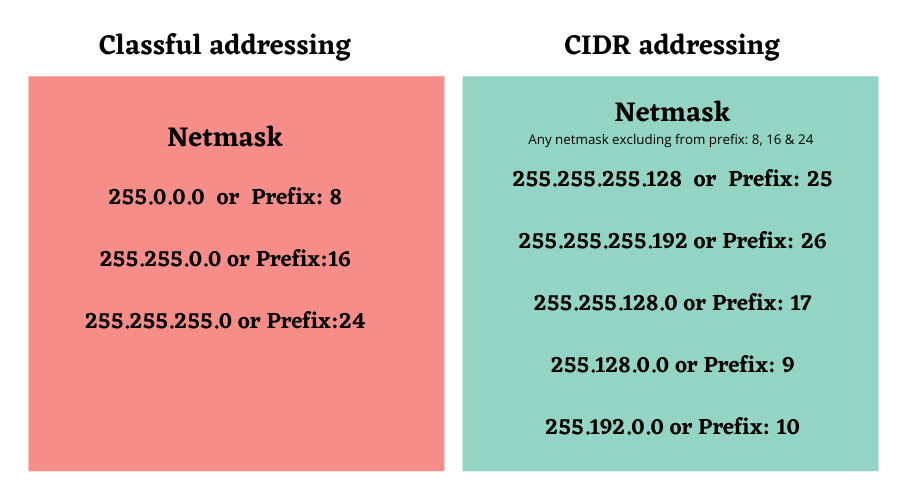
\includegraphics[scale=.55]{content/chapter14/images/cidr.png}
	\caption{Netmask as per classful \& CIDR addressing}
	\label{fig:cidr34}
\end{figure}	


	
\end{flushleft}
\newpage


